%% 
%% This is file `sample-sigchi.tex',
%% generated with the docstrip utility.
%%
%% The original source files were:
%%
%% samples.dtx  (with options: `sigchi')
%% 
%% IMPORTANT NOTICE:
%% 
%% For the copyright see the source file.
%% 
%% Any modified versions of this file must be renamed
%% with new filenames distinct from sample-sigchi.tex.
%% 
%% For distribution of the original source see the terms
%% for copying and modification in the file samples.dtx.
%% 
%% This generated file may be distributed as long as the
%% original source files, as listed above, are part of the
%% same distribution. (The sources need not necessarily be
%% in the same archive or directory.)
%%%%%%%%%%%%%%%%%%%%%%%%%%%%%%%%%%%%%%%%%%%%%%%%%%%%%%%%%%%%

%%%%%%%%%%%%%%%%%%%%%%
%%%%%% PREAMBLE %%%%%%
%%%%%%%%%%%%%%%%%%%%%%
\documentclass[sigconf,usenames,dvipsnames,svgnames,table]{acmart}

%% Packages %
  % Standard Packages %
    \usepackage{pdfpages} % Including PDFs. See Graphicx for more info
    \usepackage{amsmath}  % \mvert and other relation symbol
    \usepackage{amssymb}  % Semantic delta=
    \usepackage{amsthm}   % \begin{proof} and related sections
    \usepackage{xspace}   % Spacing for sysname
    \usepackage{dsfont}   % Fancy set letters
    \usepackage{xcolor}   % Things that need attention, and listingsconfig
  % Coding Packages %
    \usepackage{listings}
% \usepackage{sectsty}

\lstdefinelanguage{myC}{
  language=C,
  basicstyle=\ttfamily\singlespacing,
  showspaces=false,              
  showstringspaces=false,        
  showtabs=false,    
  tabsize=2,                      % sets default tabsize to 2 spaces
  captionpos=b,                   % sets the caption-position to bottom
  breaklines=true,                % sets automatic line breaking
  breakatwhitespace=false,
  escapeinside={\%*}{*)},        
  keywordstyle=\bfseries\color{black},    % keyword style
  numberstyle=\tiny\color{gray},
%  numbers=left,
%  frame=single,                  % adds a frame around the code
%  rulecolor=\color{black},
%  stepnumber=1,                 
%  numbersep=5pt,                
%  backgroundcolor=\color{white}, 
%  commentstyle=\color{dkgreen},  % comment style
%  stringstyle=\color{mauve},     % string literal style
}
% A version of the above myC, but without singlespacing
\lstdefinelanguage{myinlineC}{
  language=myC,
  basicstyle=\ttfamily
}
\renewcommand{\ttdefault}{pcr}    % enables bold monospaced font
\lstdefinelanguage[x86gasm]{Assembler}[x86masm]{Assembler}{%
,basicstyle=\ttfamily\singlespacing
,morekeywords={rax,rbx,rcx,rdx,rip,rdi,rsi,rsp,subq,decl,movq
              ,movl,xorl,imull,popq,popl,pushl}%
,morekeywords=[2]{.file,.section,.string,.text,.globl,.cfi_startproc
                 ,.cfi_def_cfa_offset,.cfi_endproc,.size,.ident}%
}
%% \definecolor{cmmtcolor}{named}{DarkGreen}
\definecolor{cmmtcolor}{named}{OliveGreen}
\lstdefinelanguage{Coq}{
,morekeywords={match,end,Definition,Inductive,Lemma,Theorem,Record,
               Hypothesis,Variable,Section,End,case,of,if,then,else,is,let,in,do,return,with,Extract,Constant,Inlined,Inline,Extraction,Fixpoint,Program,Function,Fix,Class,Local,Output,Input}
,morecomment=[s]{(*}{*)}
,keywordstyle=\bfseries\color{MidnightBlue}
,commentstyle={\color{cmmtcolor}}
,basicstyle=\sffamily
,columns=fullflexible
,numberstyle=\tiny\color{gray}
,escapeinside={@}{@}
,literate=
    {:=}{{$\defeq\;$}}1
    {<-}{{$\leftarrow\;$}}1
    {=>}{{$\Rightarrow\;$}}1
    {->}{{$\rightarrow\;$}}1
    {<->}{{$\leftrightarrow\;$}}1
    {<==}{{$\leq\;$}}1
    {\\/}{{$\vee\;$}}1
    {/\\}{{$\land\;$}}1
    {ffun}{{$\mathsf{ffun}$}}1    
    {fun}{{$\lambda$}}1
    {forall}{{$\forall$}}1
    {exists}{{$\exists$}}1
    {Z}{{$\mathbb{Z}$}}1
    {Z0}{{$\mathbb{Z}_0$}}1
    {<=}{{$\leq\;$}}1
    {>=}{{$\geq\;$}}1
    {<>}{{$\neq\;$}}1                
}

%% Verilog
\definecolor{vgreen}{RGB}{104,180,104}
\definecolor{vblue}{RGB}{49,49,255}
\definecolor{vorange}{RGB}{255,143,102}

\lstdefinestyle{verilog-style}
{
    language=Verilog,
    basicstyle=\small\sffamily,
    keywordstyle=\bfseries\color{MidnightBlue},
    identifierstyle=\color{black},
    commentstyle=\color{cmmtcolor},
    tabsize=8,
    moredelim=*[s][\colorIndex]{[}{]},
    literate=*{:}{:}1
}

\makeatletter
\newcommand*\@lbracket{[}
\newcommand*\@rbracket{]}
\newcommand*\@colon{:}
\newcommand*\colorIndex{%
   \edef\@temp{\the\lst@token}%
        \ifx\@temp\@lbracket \color{black}%
            \else\ifx\@temp\@rbracket \color{black}%
                \else\ifx\@temp\@colon \color{black}%
                    \else \color{vorange}%
                        \fi\fi\fi
                        }
\makeatother
                        

    \lstset{language=Coq}
    \usepackage[framemethod=TikZ]{mdframed}
    \mdfsetup{frametitlealignment=\center}
  % Figure Packages %
    \usepackage{caption}  % Captions
    \usepackage{framed}   % Shaded figures
    % \usepackage{epsfig}   % Import PNG figure
    \usepackage{stmaryrd} % Semantics [[ and ]]
  % Specific Thesis Packages %
    \usepackage{contour}
    \usepackage{geometry}
    \usepackage{indentfirst} % Indent after declaring a new (sub)section
    \usepackage[toc,page]
               {appendix} % Add appendix to ToC
    % \usepackage{fontenc}
    % \usepackage{setspace} % Set line spacing
    \usepackage{soul}     % Set highlight colors
    % \usepackage{tocloft}  % Set up Tables of other things
    % \usepackage{fontspec} % Specify Font
    % \usepackage{ragged2e} % Justification
  % Extra %
    % \usepackage{enumitem}
    % \usepackage{tabularx}
    % \usepackage{graphicx}
    % \usepackage{proof}  % To write Proofs (included with amsthm?)

% Custom Colors %
  % For ``shaded'' environments
    \definecolor{MyLightGrey}{gray}{.75}
    \definecolor{shadecolor}{named}{MyLightGrey} 

% Custom Definitions %
  \newcommand{\interp}[1]{\llbracket #1 \rrbracket}
  \newcommand{\shdtt}[1]{\sethlcolor{MyLightGrey}\texttt{\hl{#1}}}
  \newcommand{\obf}[1]{#1^\mathbf{o}}
  \def \sysname {\textsc{G2}\xspace}
  \def \oldname {\textsc{GARUDA}\xspace}
  \def \defeq   {\triangleq}
  \def \bksl    {\textbackslash}
  \def \latex   {\LaTeX\xspace}

%%
%% \BibTeX command to typeset BibTeX logo in the docs
\AtBeginDocument{%
  \providecommand\BibTeX{{%
    \normalfont B\kern-0.5em{\scshape i\kern-0.25em b}\kern-0.8em\TeX}}}

%% Rights management information.  This information is sent to you
%% when you complete the rights form.  These commands have SAMPLE
%% values in them; it is your responsibility as an author to replace
%% the commands and values with those provided to you when you
%% complete the rights form.
\acmConference[TODO????]{JETC Special Issue on Emerging Challenges and Solutions in Hardware Security}{15 June 2020}{????}
\setcopyright{acmcopyright}
\copyrightyear{2020}
\acmYear{2020}
% \acmDOI{10.1145/1122445.1122456}

%%
%% Submission ID.
%% Use this when submitting an article to a sponsored event. You'll
%% receive a unique submission ID from the organizers
%% of the event, and this ID should be used as the parameter to this command.
%%\acmSubmissionID{123-A56-BU3}

%%
%% The majority of ACM publications use numbered citations and
%% references.  The command \citestyle{authoryear} switches to the
%% "author year" style.
%% \citestyle{acmauthoryear}

%%
%% end of the preamble, start of the body of the document source.
\begin{document}



%% These commands are for a PROCEEDINGS abstract or paper.
% \acmConference[Woodstock '18]{Woodstock '18: ACM Symposium on Neural
%   Gaze Detection}{June 03--05, 2018}{Woodstock, NY}
% \acmBooktitle{Woodstock '18: ACM Symposium on Neural Gaze Detection,
%   June 03--05, 2018, Woodstock, NY}
% \acmPrice{15.00}
% \acmISBN{978-1-4503-XXXX-X/18/06}

%%
%% The "title" command has an optional parameter,
%% allowing the author to define a "short title" to be used in page headers.
\title{\sysname}

%%
%% The "author" command and its associated commands are used to define
%% the authors and their affiliations.

%%Check name legality.
\author{Sage Sefton}
\email{ss557415@ohio.edu}
\affiliation{%
  \institution{Ohio University}
}

\author{Avinash Karanth}
  \email{karanth@ohio.edu}
\affiliation{
  \institution{Ohio University}
%   \city{Athens}
%   \state{Ohio}
%   \postcode{45701}
}


%%
%% By default, the full list of authors will be used in the page
%% headers. Often, this list is too long, and will overlap
%% other information printed in the page headers. This command allows
%% the author to define a more concise list
%% of authors' names for this purpose.
\renewcommand{\shortauthors}{Sefton and Karanth}

\begin{abstract}

Runtime monitors to enforce processor security policies are a widely researched field.
Many systems tackle particular issues such as non-interference, cache side-channel attacks, or speculation exploits \cite{2017secverilogbl, 2019stt}.
As the attack model is ever-mutating and often undetected, these solutions can only ever solve part of the problem.
Some solutions propose generic monitors based on programmable hardware monitors \cite{2014pump} or languages for describing arbitrary policies \cite{2018garuda, 2014netkat}.
We build on the idea of verifiable policy design and empower \oldname to support Speculative and Out-of-Order Processors.
The benefits of Speculative and OOP microarchitectures are one of the most significant advancements in recent latency-mitigation research.
\sysname benefits from a refined information model and taint tracking, implemented without changes to the language itself.
These additions incur marginal processor overhead, and ring true to the spatial and power efficiency goals of the past.
We inject monitors into only one part of the processor and automate the comparator for a more streamlined design.
Finally, we will release this code, compiler, and language on GitHub.

\end{abstract}

%%%%%%%%%%%%%%%%%%%%%%%%%
%%% BEGIN             %%%
%%% TABLE OF CONTENTS %%%
%%%%%%%%%%%%%%%%%%%%%%%%%
%%% This will probably be removed at a later date,
%%% but it allows for easier navication now.
  \addcontentsline{toc}{section}{Contents}
  \tableofcontents
%%%%%%%%%%%%%%%%%%%%%%%%%
%%% END               %%%
%%% TABLE OF CONTENTS %%%
%%%%%%%%%%%%%%%%%%%%%%%%%

%%
%% The code below is generated by the tool at http://dl.acm.org/ccs.cfm.
%% Please copy and paste the code instead of the example below.
% %%
% \begin{CCSXML}
% <ccs2012>
%    <concept>
%        <concept_id>10010583.10010717.10010721</concept_id>
%        <concept_desc>Hardware~Functional verification</concept_desc>
%        <concept_significance>500</concept_significance>
%        </concept>
%    <concept>
%        <concept_id>10010583.10010682.10010689</concept_id>
%        <concept_desc>Hardware~Hardware description languages and compilation</concept_desc>
%        <concept_significance>300</concept_significance>
%        </concept>
%    <concept>
%        <concept_id>10010583.10010786.10010787.10010789</concept_id>
%        <concept_desc>Hardware~Emerging languages and compilers</concept_desc>
%        <concept_significance>500</concept_significance>
%        </concept>
%    <concept>
%        <concept_id>10010520.10010521.10010522.10010526</concept_id>
%        <concept_desc>Computer systems organization~Pipeline computing</concept_desc>
%        <concept_significance>100</concept_significance>
%        </concept>
%    <concept>
%        <concept_id>10002978.10003001.10003002</concept_id>
%        <concept_desc>Security and privacy~Tamper-proof and tamper-resistant designs</concept_desc>
%        <concept_significance>500</concept_significance>
%        </concept>
%    <concept>
%        <concept_id>10002978.10003001.10003599.10011621</concept_id>
%        <concept_desc>Security and privacy~Hardware-based security protocols</concept_desc>
%        <concept_significance>500</concept_significance>
%        </concept>
%  </ccs2012>
% \end{CCSXML}

% \ccsdesc[500]{Hardware~Functional verification}
% \ccsdesc[300]{Hardware~Hardware description languages and compilation}
% \ccsdesc[500]{Hardware~Emerging languages and compilers}
% \ccsdesc[100]{Computer systems organization~Pipeline computing}
% \ccsdesc[500]{Security and privacy~Tamper-proof and tamper-resistant designs}
% \ccsdesc[500]{Security and privacy~Hardware-based security protocols}

%%
%% Keywords
\keywords{hardware security, software verification, memory obfuscation}

%%
%% This command processes the author and affiliation and title
%% information and builds the first part of the formatted document.
\maketitle
%%%%%%%%%%%%%%%%%%%%%%%
%%% BEGIN SECTION 1 %%%
%%% INTRODUCTION    %%%
%%%%%%%%%%%%%%%%%%%%%%%
  \section{Introduction}\label{sec:intro}
    \sysname Intro
    \cite{2011gem5sim}
    \cite{2019stt}
    The rest of this thesis loosely follows a standard academic journal submission's organization.
    Section~\ref{sec:priorwork} summarizes a prior attack models and their proposed solutions.
    The \sysname language is described in detail in Section~\ref{sec:spec} and is demonstrated in Section~\ref{sec:proofs}.
    Section~\ref{sec:compile} describes the intermediate steps towards the compilation of \sysname into Verilog.
    Research done since this paper's release are shown in Section~\ref{sec:more}.
    Sections~\ref{sec:conclude} and~\ref{sec:coauthor} conclude and cite the work done by my colleagues and advisors.
%%%%%%%%%%%%%%%%%%%%%
%%% END SECTION 1 %%%
%%% INTRODUCTION  %%%
%%%%%%%%%%%%%%%%%%%%%

%%%%%%%%%%%%%%%%%%%%%%%
%%% BEGIN SECTION 2 %%%
%%% PRIOR WORK      %%%
%%%%%%%%%%%%%%%%%%%%%%%
  \section{Prior Work}\label{sec:priorwork}
    \begin{table}
      \centering
      \begin{tabular}{|c|l|l|} 
        \hline
          & Rumtime Monitors & Compiler Enforcements\\
        \hline
          Advantages
          & - Often programmable 
            & - Low Overhead \\
          & - Can trigger exceptions or
            & - Possible violations detected \\
          &\quad OS traps &\quad before synthesis \\ 
          & - Modular, not application  
            & - Violations during runtime \\
          &\quad specific &\quad simply fail \\
          \hline
          Disadvantages
          & - Exceptions and traps are slow 
            & - Static after synthesis \\
          & - Larger overhead 
            & - Violation-response is static \\
          & &\quad and defined at compile time \\
        \hline
      \end{tabular}
      \caption{Comparison of Runtime Monitors and Compile-Time Enforcement.}
      \label{table:prior:run-vs-comp}
    \end{table}

%%%%%%%%%%%%%%%%%%%%%
%%% END SECTION 2 %%%
%%% PRIOR WORK    %%%
%%%%%%%%%%%%%%%%%%%%%

  
%%%%%%%%%%%%%%%%%%%%%%
%%% BEGIN SECTON 3 %%%
%%% SYSTEM SPECS   %%%
%%%%%%%%%%%%%%%%%%%%%%
  \section{The Implementation of \sysname}\label{sec:spec}
    % \oldname was initially designed with the goal of making the definitions of security policies available to more users.
    % Hardware policy enforcement was largely relegated to those who understood hardware and the languages used to describe it.
    % All of the compiled extensions to Verilog, by definition, require the engineer to have an understanding of Verilog itself.
    % In addition, the author of a security policy would have a difficult time verifying if that policy functioned as intended.
    % Does their policy \textit{verifiably} work for all possible cases, or have they missed an edge case that could become the next Spectre or Meltdown~\cite{2018spectre, 2018meltdown}?
    % \par
    
    %%%%%%%%%%%%%%%%%%%%%%%%%
    %%% BEGIN SECTION 3.1 %%%
    %%% SYSTEM SYNTAX     %%%
    %%%%%%%%%%%%%%%%%%%%%%%%%
    \subsection{Syntax}\label{sec:spec:synt}
      We start by defining the syntax of \sysname.
      As our language is derived from KAT, this definition may be familiar to some readers.
   
      %%%%%%%%%%%%%%%%%%%%%%%%%%%
      %%% BEGIN SECTION X.1.1 %%%
      %%% SYSTEM DEFINITIONS  %%%
      %%%%%%%%%%%%%%%%%%%%%%%%%%%
      \subsubsection{Definitions}\label{sec:spec:synt:defn}
        First we define the equivalents of boolean variables to our language in Figure~\ref{fig:spec:synt:defn}.
        In the same way a boolean algebra would define a boolean variable to belong to the set $\{0 \mid 1\}$, we define what it means for a variable to be a field, instruction, or result.
        Generic fields $f$ are defined as either an Instruction Field or a Result Field.
        Instruction fields are the variables that represent instructions.
        In a statement \shdtt{$f_{i_{1}} =$ \textbf{ADD} x1 x2 x3}, the \textit{field} would be \shdtt{$f_{i_{1}}$}.
        Result fields are the same, except they are denoted with an 'r': \shdtt{$f_{r_{1}}$}.
        Instructions and Results follow a similar convention, and we have already defined one.
        The string \shdtt{$f_{i_{1}} =$ \textbf{ADD} x1 x2 x3} is an instruction itself, where the machine code is just \shdtt{\textbf{ADD} x1 x2 x3}.

        % Definitions table
        \begin{figure}
          \centering
          \begin{tabular}{l l c l}
            EXE Input Fields & $f_{Ei}$  & $::=$ & $f_{Ei_{1}} \mid \dots \mid f_{Ei_{k}}$\\
            State Reg Fields & $f_{SR}$  & $::=$ & $f_{SR_{1}} \mid \dots \mid f_{SR_{k}}$\\
            MEM Input Fields & $f_{Mi}$  & $::=$ & $f_{Mi_{1}} \mid \dots \mid f_{Mi_{k}}$\\
            Fields           & $f$       & $::=$ & $f_{Ei} \mid f_{SR} \mid f_{Mi} $ \\
            Obfuscated Field & $\obf{f}$ & $::=$ & $f$\\
            Inputs           & $i$       & $::=$ & $\{f_{i_{1}} = v_{i_{1}} ,\ \dots\ ,\ f_{i_{k}} = v_{i_{k}}\}$\\
            Outputs          & $o$       & $::=$ & $\{f_{o_{1}} = v_{o_{1}} ,\ \dots\ ,\ f_{o_{k}} = v_{o_{k}}\}$\\
            Obfuscation Fxn  & $\Phi$    & $::=$ & $f \rightarrow \obf{f} \mid \obf{f} \rightarrow f$
            % TODO: how do we define state in and state out? -- Who cares?  that's not part of the language
            % TODO: Mention that Inputs and Outputs can generically refer to either EXE or MEM.
            %       Indeed, the Outputs refers to both.
          \end{tabular}
          \caption{Definitions in \sysname.}
          \label{fig:spec:synt:defn}
        \end{figure}

      %%%%%%%%%%%%%%%%%%%%%%%%%%%%
      %%% BEGIN SECTION 3.1.2  %%%
      %%% SYNTAX OF PREDICATES %%%
      %%%%%%%%%%%%%%%%%%%%%%%%%%%%
      \subsubsection{Syntax of Predicates}\label{sec:spec:synt:pred}
        After the variables are defined, we move on to the \textit{Predicates}.
        The predicate language is how a programmer designs a test.
        Upon first glance at Figure~\ref{fig:spec:synt:pred}, most viewers may see this as just a representation of a boolean algebra.
        In fact, as touched upon in Section~\ref{sec:prior:ka:kat}, the predicate language is exactly a boolean algebra.
        The only potential difference is the \textit{Test} field, which is just a way to turn a field's value into a boolean one.
        The field \shdtt{$f_i$} is clearly not a boolean variable, but \shdtt{$f_i = f_i$} is\footnote{Most languages see this as an assignment.  In \sysname, assignments are done with the $\leftarrow$.}.
        Note that we define the variables \shdtt{$a, b$} to be predicate placeholders.
        These variables are used as a shorthand in our Extended BNF~\cite{ISO14977} specifications.
        Otherwise, we would have to write \textit{<Predicates>} every time we wanted to reference this type.
        % Predicates table
        \begin{figure}
          \centering
          \begin{tabular}{l c r l l}
            Predicates  & $a,b$ & $::=$  & $0$          & \textit{False}    \\
                        &       & $\mid$ & $1$          & \textit{Identity} \\
                        &       & $\mid$ & $f = n$      & \textit{Test}     \\
                        &       & $\mid$ & $a + b$      & \textit{Sum}      \\
                        &       & $\mid$ & $a \cdot b$  & \textit{Product}  \\
                        &       & $\mid$ & $\neg\ a$    & \textit{Negation}
          \end{tabular}
          \caption{Predicates in \sysname act as a boolean algebra.}
          \label{fig:spec:synt:pred}
        \end{figure}

      %%%%%%%%%%%%%%%%%%%%%%%%%%%
      %%% BEGIN SECTION 3.1.3 %%%
      %%% SYNTAX OF POLICIES  %%%
      %%%%%%%%%%%%%%%%%%%%%%%%%%%
      \subsubsection{Syntax of Policies}\label{sec:spec:synt:pol}
        \textit{Policies} are quite a bit more complicated than predicates.
        The policy language is an augmentation of a Kleene algebra, where all the primitives are relevant to the monitor theory presented in Section~\ref{sec:prior:mon}.
        The formal definition of all these policies are found in Figure ~\ref{fig:spec:synt:pol}.
        \par

        The \textit{Test} rule is very similar to the same one in Figure~\ref{fig:spec:synt:pred}.
        It is the \textit{Test} part of a Kleene algebra with tests.
        Scripting programmers may see this as the equivalent of an \shdtt{if} statement, which is accurate.
        If the predicate \shdtt{$a$} in \shdtt{$\mathbf{test}(a)$} evaluates to the \textit{Identity}, the equivalent scripting functionality would be a satisfied \shdtt{if} statement.
        In \oldname, this means that the evaluation of the policy can continue.
        The actual function of this is explained in far more detail in Section~\ref{sec:spec:sem:pol}.
        \par
        
        \textit{Injection Action} and \textit{Injection Result} are just methods of inserting their respective fields.
        Say the policy engineer would like to return a zero instead of whatever the actual computed value was, \textit{Injection Result} would be the correct tool.
        \par

        We come to the final three policy rules, by far the most complex and powerful.
        \textit{Update}, as briefly mentioned earlier, uses the $\leftarrow$ operator.
        This rule is analogous to assigning a value to a variable.
        While this is a simple idea, the implementation of such an action is fairly complex.
        \textit{Choice} is the policy-equivalent to a predicate \textit{Sum}.
        When the monitor comes across a choice, both sub-policies must be evaluated in parallel.
        Either, both, or neither may apply to the current state of the machine.
        Finally, \textit{Sequential Concatenation} is the way a programmer can assign a series of tests, policies, or otherwise.
        Our monitor cannot look ahead or to past instructions, but it can keep track of its own state.
        If the user wanted to create a policy that satisfies whenever a load \textit{and then} a branch occurs, they would use this rule.
        Simply write two predicates for each test, and then concatenate them with the \shdtt{$\cdot$}.

        % Policies table
        \begin{figure}
          \centering
          \begin{tabular}{l c r l l}
            Policies  & $p,q$ & $::=$  & $\mathbf{test}(a)$ & \textit{Test}           \\
                      &       & $\mid$ & $(\Phi_{Encrypt},$ &                         \\
                      &       &        &\ $\Phi_{Decrypt})$ & \textit{Obfuscation}    \\
                      &       & $\mid$ & $inj_{Rs}$         & \textit{Injection to}   \\
                      &       &        &                    & \textit{State Register} \\
                      &       & $\mid$ & $inj_{Mi}$         & \textit{Inject to}      \\
                      &       &        &                    & \textit{Memory Unit}    \\
                      &       & $\mid$ & $f \leftarrow n$   & \textit{Update}         \\
                      &       & $\mid$ & $p + q$            & \textit{Choice}         \\
                      &       & $\mid$ & $p \cdot q$        & \textit{Sequential}     \\
                      &       &        &                    & \textit{Concatenation}  \\
          \end{tabular}
          \caption{Syntax of Policies in \sysname}
          \label{fig:spec:synt:pol}
        \end{figure}



    %%%%%%%%%%%%%%%%%%%%%%%%%
    %%% BEGIN SECTION 3.2 %%%
    %%% SYSTEM SEMANTICS  %%%
    %%%%%%%%%%%%%%%%%%%%%%%%%
    \subsection{Semantics}\label{sec:spec:sem}
      Here we define what each of the syntactic rules described above actually mean.
      In effect, this is a translation of the language into what the monitor can do for any given input.
      As mentioned, we have a monitor that operates on two streams.
      To visualize a machine that operates on streams, the analogy of an older dot-matrix printer can be used.
      Many of my readers may not be familiar with this technology, so I provide a simplified version of this kind of printer in Figure~\ref{fig:spec:sem:sprint}.
      With these kinds of printers, the paper comes perforated between every page.
      All of the pages are connected and the stack is folded in a zig-zag.
      There are guides on the sides of the papers, which act as their margins and assist the printer in moving the paper through its system.
      The important thing to note about these kinds of printers is that they are continuous; there is always a stream of non-interruptable inputs \footnote{For simplicity, assume an infinite spool of this paper}.
      This printer is a useful analogy of a single-stream machine.
      \par

      If we bring the context back to \oldname, we must use Figure~\ref{fig:spec:sem:dprint}.
      This image depicts a printer with two streams of paper, with the outputs for each on opposite sides.
      \oldname operates in this way, and I have labeled the instruction and result streams accordingly.
      The blank paper feeding into the input side of this printer can be thought of as the instructions being sent to the CPU.
      \oldname is given an opportunity to modify, or ``print'' on, this stream.
      The inputs stream exits the printer, is processed by the CPU, and returns the results stream.
      This stream can be modified as well by the exact same device that also processed the inputs.
      Unifying the input and output processing in this way means that communication, and thus decision making, is easier for complex stream processing.
      \par

      For how the \textit{language} of \oldname works, we have to refer to the theory of regular expressive languages from Section~\ref{sec:prior:ka:star}.
      Recall that a regular expression, when compiled, returns a set of all possible satisfying strings.
      For our purposes, we don't just look at satisfactory strings, but satisfactory \textit{streams} of strings.
      We represent these streams as a set of all possible combinations of inputs.
      Processing a regular expression over a standard alphabet of characters produces strings, but our input is no longer an alphabet of characters.
      A regular expression that accepts all strings returns the \textit{Power Set} of the input alphabet.
      Indeed, you can see in Figure~\ref{fig:spec:sem:pred} that the first entry is what the interpretation operator \shdtt{$\interp{\cdot}$}
      \footnote{The dot seen in the middle of the \shdtt{$\interp{}$} operator acts as a placeholder.
      In this case, it is NOT a Sequential Concatenation.} means.
      A similar policy that accepts all possible inputs returns the power set of the input and output streams \shdtt{$P(\mathbf{Stream}(E))\times P(\mathbf{Stream}(M))$}.

      % \begin{figure}
      %   \centering
      %   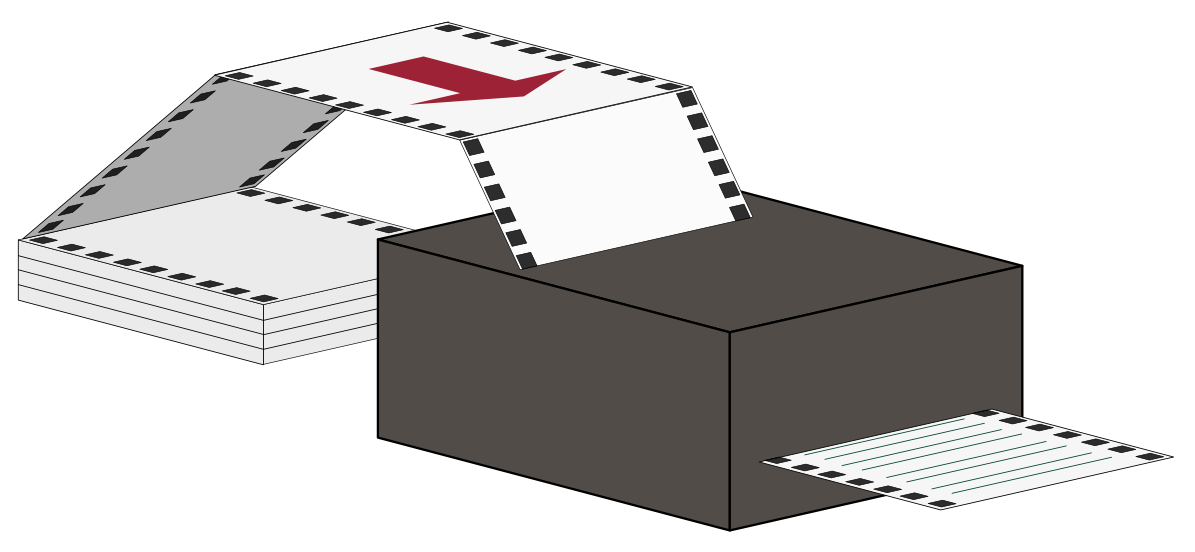
\includegraphics[width=0.4\textwidth]{sprint.png}
      %   \caption{An older, continuous feed printer.}
      %   \label{fig:spec:sem:sprint}
      % \end{figure}

      % \begin{figure}
      %   \centering
      %   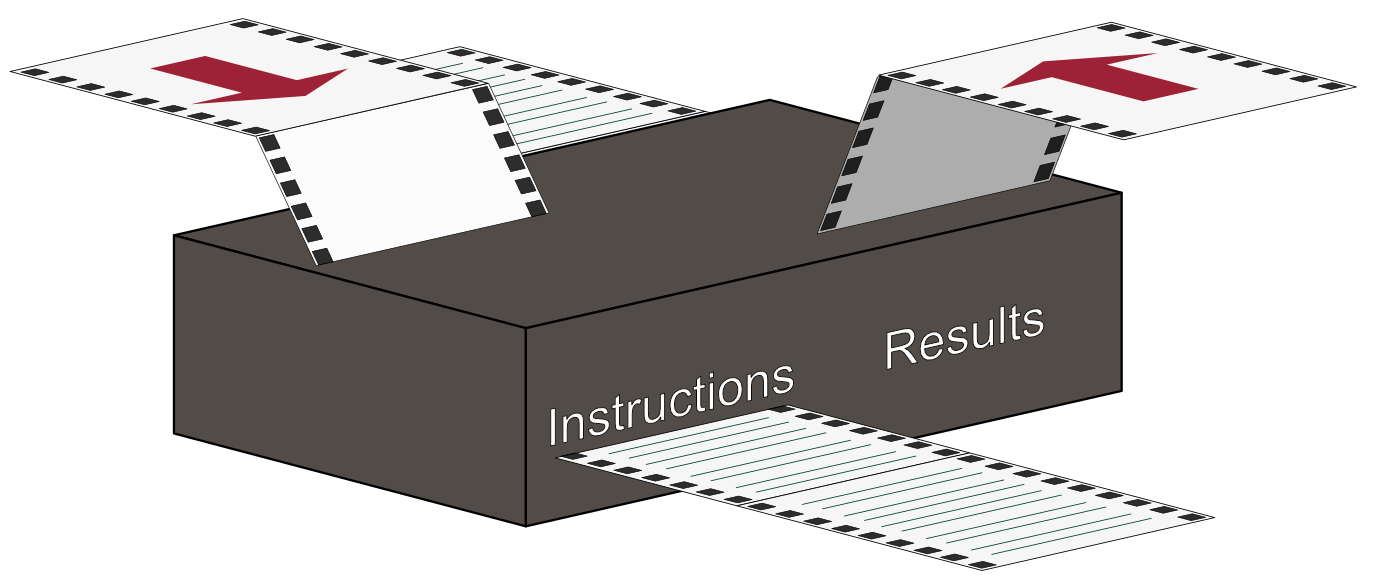
\includegraphics[width=0.4\textwidth]{dprint.png}
      %   \caption{The monitor used in \oldname, demonstrated as a printer operating on two continuous feeds of paper.}
      %   \label{fig:spec:sem:dprint}
      % \end{figure}
      %%%%%%%%%%%%%%%%%%%%%%%%%%%%%
      %%% BEGIN SECTION 3.2.1   %%%
      %%% SEMANTICS: PREDICATES %%%
      %%%%%%%%%%%%%%%%%%%%%%%%%%%%%
      \subsubsection{Semantics of Predicates}\label{sec:spec:sem:pred}

        % Semantics of Predicates
        \begin{figure}
          \centering
          { %\fontsize{8pt}{10pt}
          \begin{align*}
            % Theory
            \interp{ \cdot }\ 
              :\ \ &
              \mathbf{Stream}(E)\times \mathbf{Stream}(M) \rightarrow \\
              & P(\mathbf{Stream}(E))\times P(\mathbf{Stream}(M)) 
              \\\hline
            % Falsity
            \interp{ 0 }(-, -)
              \triangleq\ &
              (\emptyset , \emptyset)
              \\ % or null-stream?
            % Identity
            \interp{ 1 }(es, ms)
              \triangleq\ &
              (\{es\},\{ms\})
              \\
            % Test
            \interp{ f=n }(es, ms)
              \triangleq\ &
                (\mathsf{filter}\ (f=n)\ \{es\},\\
              &\ \mathsf{filter}\ (f=n)\ \{ms\}) 
              \\
            % Sum
            \interp{ a + b }(es, ms)
              \triangleq\ &
              \interp { a }(es, ms)\cup
              \interp { b }(es, ms) \\
              &\mathsf{where}\ 
                (S_e^1, S_m^1)\cup (S_e^2, S_m^2)\triangleq\\
                &\quad\quad\ \ \ 
                (S_e^1\cup S_e^2, S_m^1\cup S_m^2)\\
            % Product
            \interp { a \cdot b }(es, ms)
              \triangleq\ &
              \interp { a }(es, ms)\cap
              \interp { b }(es, ms) \\
              &\mathsf{where}\ 
                (S_e^1, S_m^1)\cap (S_e^2, S_m^2)\triangleq\\
                &\quad\quad\ \ \ 
                (S_e^1\cap S_e^2, S_m^1\cap S_m^2)\\
            % Negation
            \interp { \neg a }(es, ms)
              \triangleq\ &
              \mathsf{let}\ (S_e, S_m) = \interp {a}(es, ms) \\
              &\mathsf{in}\ (\{es\} - S_e, \{ms\} - S_m)
              \\
          \end{align*}}
          \caption{The semantics of predicates in \sysname.  While predicates remain unchanged from \oldname, the theory changes slightly}
          \label{fig:spec:sem:pol}
        \end{figure}

      %%%%%%%%%%%%%%%%%%%%%%%%%%%
      %%% BEGIN SECTION 3.2.2 %%%
      %%% SEMANTICS: POLICIES %%%
      %%%%%%%%%%%%%%%%%%%%%%%%%%%
      \subsubsection{Semantics of Policies}\label{sec:spec:sem:pol}
        \begin{figure}
          \centering
          { %\fontsize{8}{10}
          \begin{align*}
            % Theory
            \interp { \cdot }\ 
              :\ \ &
              \mathbf{Stream}(E)\times \mathbf{Stream}(M) \rightarrow \\
              & P(\mathbf{Stream}(E))\times P(\mathbf{Stream}(M)) 
              \\\hline
            % Obfuscation
            \interp {(\Phi_{En}, \Phi_{De})}(es, ms)\
              \triangleq\
              & \mathsf{let}\ (e \rightarrow \obf{e} = \Phi_{En}),\\
              & \quad\ \      (\obf{m} \rightarrow m = \Phi_{De}) \\
              % & \mathsf{let}\ e \rightarrow \obf{e} = \Phi_{Encrypt}\\
              % & \mathsf{and}\ \obf{m} \rightarrow m = \Phi_{Decrypt}\\
              & \mathsf{in}\
              (\{\obf{e}\}, \{m\})
              \\
            % Injection Action
            \interp { inj_{SR}(e) }(es, ms)
              \triangleq\ &
              (\{e : es\}, \{ms\}) 
              % or ::?  ;i sequential
              \\
            % Injection Result
            \interp { inj_{Mi}(m) }(es, ms)
              \triangleq\ &
              (\{es\},\{m : ms\})
              \\
            % Modification
            \interp { f \leftarrow n }(es, ms)
              \triangleq\ 
              & (\mathsf{map}\ (f\leftarrow n)\ \{e\},\\
              &\ \mathsf{map}\ (f\leftarrow n)\ \{m\})
              \\ %  could use editing?
            % Policy Union
            \interp { p + q }(es, ms)
              \triangleq\ &
              \interp { p }(e, m)\cup
              \interp { q }(e, m) \\
              &\mathsf{where}\ (S_e^1, S_m^1)\cup (S_e^2, S_m^2)\triangleq\\
              &\quad\quad\quad (S_e^1\cup S_e^2, S_m^1\cup S_m^2)\\
              % A union of the streams gives a nondeterministic machine.
            % Policy Concatnation
            \interp { p \cdot q }(es, ms)
              \triangleq\ &
              \mathsf{let}\ (S_e, S_m) = \interp{p}(e, m)\\
              &\mathsf{in}\ \bigcup \{\interp{q}(e',m')\ |\ e'\in S_e, m'\in S_m\}\\
              % \\
              \hline
            % Defn. of Filter
            \interp{\mathsf{filter}\ f}(S)
              \triangleq\ & \{l \in S\ |\ f(l) = \mathsf{true}\}\\
            % Defn. of Map
            \interp{\mathsf{map}\ g}(S)
              \triangleq\ &
              \{ g(l)\ |\ l\in S \} 
          \end{align*}}
          \caption{The semantics of policies in \sysname.}
          \label{fig:spec:sem:pol}
        \end{figure}

%%%%%%%%%%%%%%%%%%%%%%
%%% BEGIN SECTON 4 %%%
%%% PROOFS         %%%
%%%%%%%%%%%%%%%%%%%%%%
  \section{TODO: Name: Proofs}\label{sec:proofs}
    %%%%%%%%%%%%%%%%%%%%%%%%
    %%% BEGIN SECTON 4.0 %%%
    %%% WHY PROOFS       %%%
    %%%%%%%%%%%%%%%%%%%%%%%%

    %%%%%%%%%%%%%%%%%%%%%%%%
    %%% BEGIN SECTON 4.1 %%%
    %%% NO OBFUSCATION   %%%
    %%%%%%%%%%%%%%%%%%%%%%%%
    %%% Demonstrate the basic flow of a policy

    %%%%%%%%%%%%%%%%%%%%%%%%
    %%% BEGIN SECTON 4.2 %%%
    %%% XOR KEY          %%%
    %%%%%%%%%%%%%%%%%%%%%%%%
    %%% Demonstrate proofs on converse PhiOps

    %%%%%%%%%%%%%%%%%%%%%%%%
    %%% BEGIN SECTON 4.3 %%%
    %%% SOMETHING ABOUT PHI STACKING ??? %%%
    %%%%%%%%%%%%%%%%%%%%%%%%
    %%% Demonstrate complex policy decision making


    %%%%%%%%%%%%%%%%%%%%%%%%
    %%% BEGIN SECTON 4.1 %%%
    %%% EXAMPLE ATTACKS  %%%
    %%%%%%%%%%%%%%%%%%%%%%%%
    %%% Demonstrate a thwarted attack

%%%%%%%%%%%%%%%%%%%%%%%%
%%% BEGIN SECTON 5   %%%
%%% FULL COMPILATION %%%
%%%%%%%%%%%%%%%%%%%%%%%%
  \section{Compilation to Verilog}\label{sec:comp}
    Label Test: 
    ~\ref{sec:comp:int}
    ~\ref{sec:comp:comp}
    ~\ref{sec:comp:comp:pred}
    ~\ref{sec:comp:comp:pol}
    ~\ref{fig:comp:int}
    ~\ref{tab:comp:comp:ports}
    ~\ref{fig:comp:comp:pred}
    ~\ref{fig:comp:comp:pol}
    %%%%%%%%%%%%%%%%%%%%%%%%
    %%% BEGIN SECTON 5.1 %%%
    %%% INTERMEDIATE     %%%
    %%%%%%%%%%%%%%%%%%%%%%%%
    \subsection{The Intermediate Language}\label{sec:comp:int}

      \begin{figure}
        \centering
        \begin{tabular}{l r r l l}
          % Definitions table
          Values        & $v$     & $::=$     & $\mathsf{INSTR\ |\ RES}$ &\\
          Registers     & $b$     & $::=$     & $\mathsf{reg}$           &\\
          \\
          % Predicates table
          Expressions & $e$ & $::=$  & $read(b)$       
                            & \textit{Read Reg}\\
                      &     & $\mid$ & $write(b,v)$    
                            & \textit{Write Value to Reg}\\
                      &     & $\mid$ & $let\ x = e_1\ in\ e_2$ 
                            & \textit{Assignment}\\  
                      &     & $\mid$ & $e_1\ ||\ e_2$ 
                            & \textit{Parallel}\\
                      &     & $\mid$ & $f(e_1)$        
                            & \textit{Apply Function} \\  
                      &     & $\mid$ & $if\ v = n\ then\ e_1\ else\ e_2$
                            & \textit{Conditional} \\
                      &     & $\mid$ & $e_1\ \&\&\ e_2$ 
                            & \textit{Product (AND)}\\
                      &     & $\mid$ & $e_1 ; e_2$
                            & \textit{Concatenation}\\
                      &     & $\mid$ & $forever\ e$ 
                            & \textit{Hardwire}
        \end{tabular}
        \caption{The language \sysname uses as a means to facilitate compilation.}
        \label{fig:comp:int}
      \end{figure}
    %%%%%%%%%%%%%%%%%%%%%%%%
    %%% BEGIN SECTON 5.2 %%%
    %%% COMPILATION      %%%
    %%%%%%%%%%%%%%%%%%%%%%%%
    \subsection{Compiling \sysname to the Intermediate}\label{sec:comp:comp}
      We define a function $\mathbf{C}$ to be the compilation of some predicate or policy in \sysname to the intermediate language.
      $\mathbf{C}$ operates on the four ports of the \sysname monitor.
      These consist of the processing done after the Execution stage, before the Memory stage, and their respective altered streams.
      Table~\ref{tab:compile:compile:ports} summarizes each port.
      Assume all $\mathbf{C}$ are short for $\mathbf{C}_{(EXE,\obf{EXE},\obf{MEM},MEM)}$ if unspecified.
      % Would it be best to flip MEM and MEM' to show the return to the original output of EXE?
      \begin{table}
        \centering
        \begin{tabular}{c | l}
          PORT        & DESCRIPTION \\ \hline
          $EXE$       & Direct output of the execution stage. \\
          $\obf{EXE}$ & Altered state register input. \\
          $\obf{MEM}$ & Direct output of the state register. \\
          $MEM$       & Altered memory access input. 
        \end{tabular}
        \caption{
          The four ports used in compilation.
          These are the inputs and outputs for logic between the functional units and state register.
        }
        \label{tab:comp:comp:ports}
      \end{table}

      %%%%%%%%%%%%%%%%%%%%%%%%%%
      %%% BEGIN SECTON 5.2.1 %%%
      %%% PREDICATES         %%%
      %%%%%%%%%%%%%%%%%%%%%%%%%%
      \subsubsection{Compiling Predicates}\label{sec:comp:comp:pred}
        \begin{figure}
          \begin{align*}
            % Falsity
            \mathbf{C}[0]\ 
              =\ &
              let\    E\_bog = \text{new buf}\\
              &\quad\ M\_bog = \text{new buf}\\
              &in\ write(\obf{EXE}, E\_bog)\\
              &\quad  write(MEM, M\_bog)\\
            % Identity
            \mathbf{C}[1]\ 
              =\ &
              write(\obf{EXE}, read(EXE))\\
              &write(MEM, read(\obf{MEM}))
              \\
            % Filter
            \mathbf{C}[f = n]\
              =\
              &if\ EXE=n\ then\\
              &\quad write(\obf{EXE}, read(EXE))\\
              &\quad else\ \mathbf{C}_{(EXE, \obf{EXE}, -, -)}[0]\\
              &if\ \obf{MEM}=n\ then\\
              &\quad write(MEM, read(\obf{MEM}))\\
              &\quad else\ \mathbf{C}_{(-, -, \obf{MEM}, MEM)}[0]\\
            % Predicate Addition
            \mathbf{C}[\mathsf{test}(a + b)]\ 
              =\
              & (*Intermediate\ Execution\ Ports*)\\
              & let\ E_{ai}, \obf{E}_{ai}, E_{bi}, \obf{E}_{bi} = \text{new buf}\ in\\
              & (*Intermediate\ Memory\ Ports*)\\
              & let\ \obf{M}_{ai}, M_{ai}, \obf{M}_{bi}, M_{bi} = \text{new buf}\ in\\
              &\quad\ \ DeMux(EXE, E_{ai}, E_{bi})\ ||\\
              &\quad\ \ DeMux(\obf{MEM}, \obf{M}_{ai}, \obf{M}_{bi})\\
              &let\     i_a = \mathbf{C}_{(E_{ai},\obf{E}_{ai},\obf{M}_{ai},M_{ai})}[a]\\
              &\quad\ \ i_b = \mathbf{C}_{(E_{bi},\obf{E}_{bi},\obf{M}_{bi},M_{bi})}[b]\\
              &in\ Mux(i_a\ \ i_b, (\obf{EXE},MEM))\\
            % Predicate Product
            \mathbf{C}[\mathsf{test}(a \cdot b)]\ 
              =\ &\mathbf{C}[\mathsf{test}(a) \cdot \mathsf{test}(b)] \\
            % Predicate Negation
            \mathbf{C}[\neg a]\ 
              =\ 
              &if\ \neg a\ then\\
              &\quad write(\obf{EXE}, read(EXE))\\
              &\quad write(MEM, read(\obf{MEM}))\\
              &else\ \mathbf{C}[0]\\
          \end{align*}
          \caption{
            Compilation of \sysname predicates into the intermediate language.
            These remain largely unchanged from \oldname.
          }
          \label{fig:comp:comp:pred}
        \end{figure}

    %%%%%%%%%%%%%%%%%%%%%%%%%%
    %%% BEGIN SECTON 5.2.2 %%%
    %%% POLICIES           %%%
    %%%%%%%%%%%%%%%%%%%%%%%%%%
      \subsubsection{Compiling Policies}\label{sec:comp:comp:pol}
        \begin{figure}
          \begin{align*}
            % Inject Instruction
            \mathbf{C}[inj_{SR}V]\ 
              =\ &
              write(\obf{EXE}, V)\\
            % Inject Result
            \mathbf{C}[inj_{Mi}V]\ 
              =\ &
              write(MEM, V)\\
            % Assignment
            \mathbf{C}[f \leftarrow n]\ 
              =\ &
              let\    e' = f(read(EXE))\\
              &\quad\ m' = f(read(\obf{MEM}))\\
              &in\ write(\obf{EXE}, e')\\
              &\quad \ write(MEM, m')\\
            % Policy Nondeterministic Choice
            \mathbf{C}[p + q]\ 
              =\ &
              let\      e_p = \mathbf{C}[p]\\
              &\quad\ \ e_q = \mathbf{C}[q]\\
              &in\ Mux(e_p, e_q, (\obf{EXE},MEM))\\
            % Policy Sequence
            \mathbf{C}[p \cdot q]\ 
              =\ &
              let\    EXE_{mid} = \text{new buf}\\
              &\quad\ MEM_{mid} = \text{new buf}\\
              &\quad\ \ e_p = \mathbf{C}_{( EXE, EXE_{mid}, \obf{MEM}, MEM_{mid}      )}[p]\\
              &\quad\ \ e_q = \mathbf{C}_{(      EXE_{mid}, \obf{EXE}, MEM_{mid}, MEM )}[q]\\
              &in\ e_p\ ;\ e_q
          \end{align*}
          \caption{Compilation of \sysname policies into the intermediate language.}
          \label{fig:comp:comp:pol}
        \end{figure}





%%
%% The acknowledgments section is defined using the "acks" environment
%% (and NOT an unnumbered section). This ensures the proper
%% identification of the section in the article metadata, and the
%% consistent spelling of the heading.
\begin{acks}
To ...
\end{acks}

%%
%% The next two lines define the bibliography style to be used, and
%% the bibliography file.
\bibliographystyle{ACM-Reference-Format}
\bibliography{Garuda2.0}

%%
%% If your work has an appendix, this is the place to put it.
\appendix

\section{Research Methods}

\subsection{Part One}

Appendix A1

\subsection{Part Two}

Appendix A2

\section{Online Resources}

Appendix B

\end{document}
\endinput
